\section*{Experiment 2}
In this experiment, we explore how series and parallel combinations of \nMOS transistors behave, 
and what affect these combinations have on the channel current, \Isat, as a function of gate voltage,
\Vg. In order to accomplish this comparison, we collected data for the channel current in both ohmic 
and saturation regions of operation for a single \nMOS transistor, two transistors in parallel, and
two transistors in series, with the same gate, source, drain and bulk voltages. We tested the 
configurations in both the ohmic and saturation regions of operation, using $V_{gb} = 10mV$ and
 $ V_{ds} = V_{dd}$ and respectively.

\begin{figure}[H]
\centering
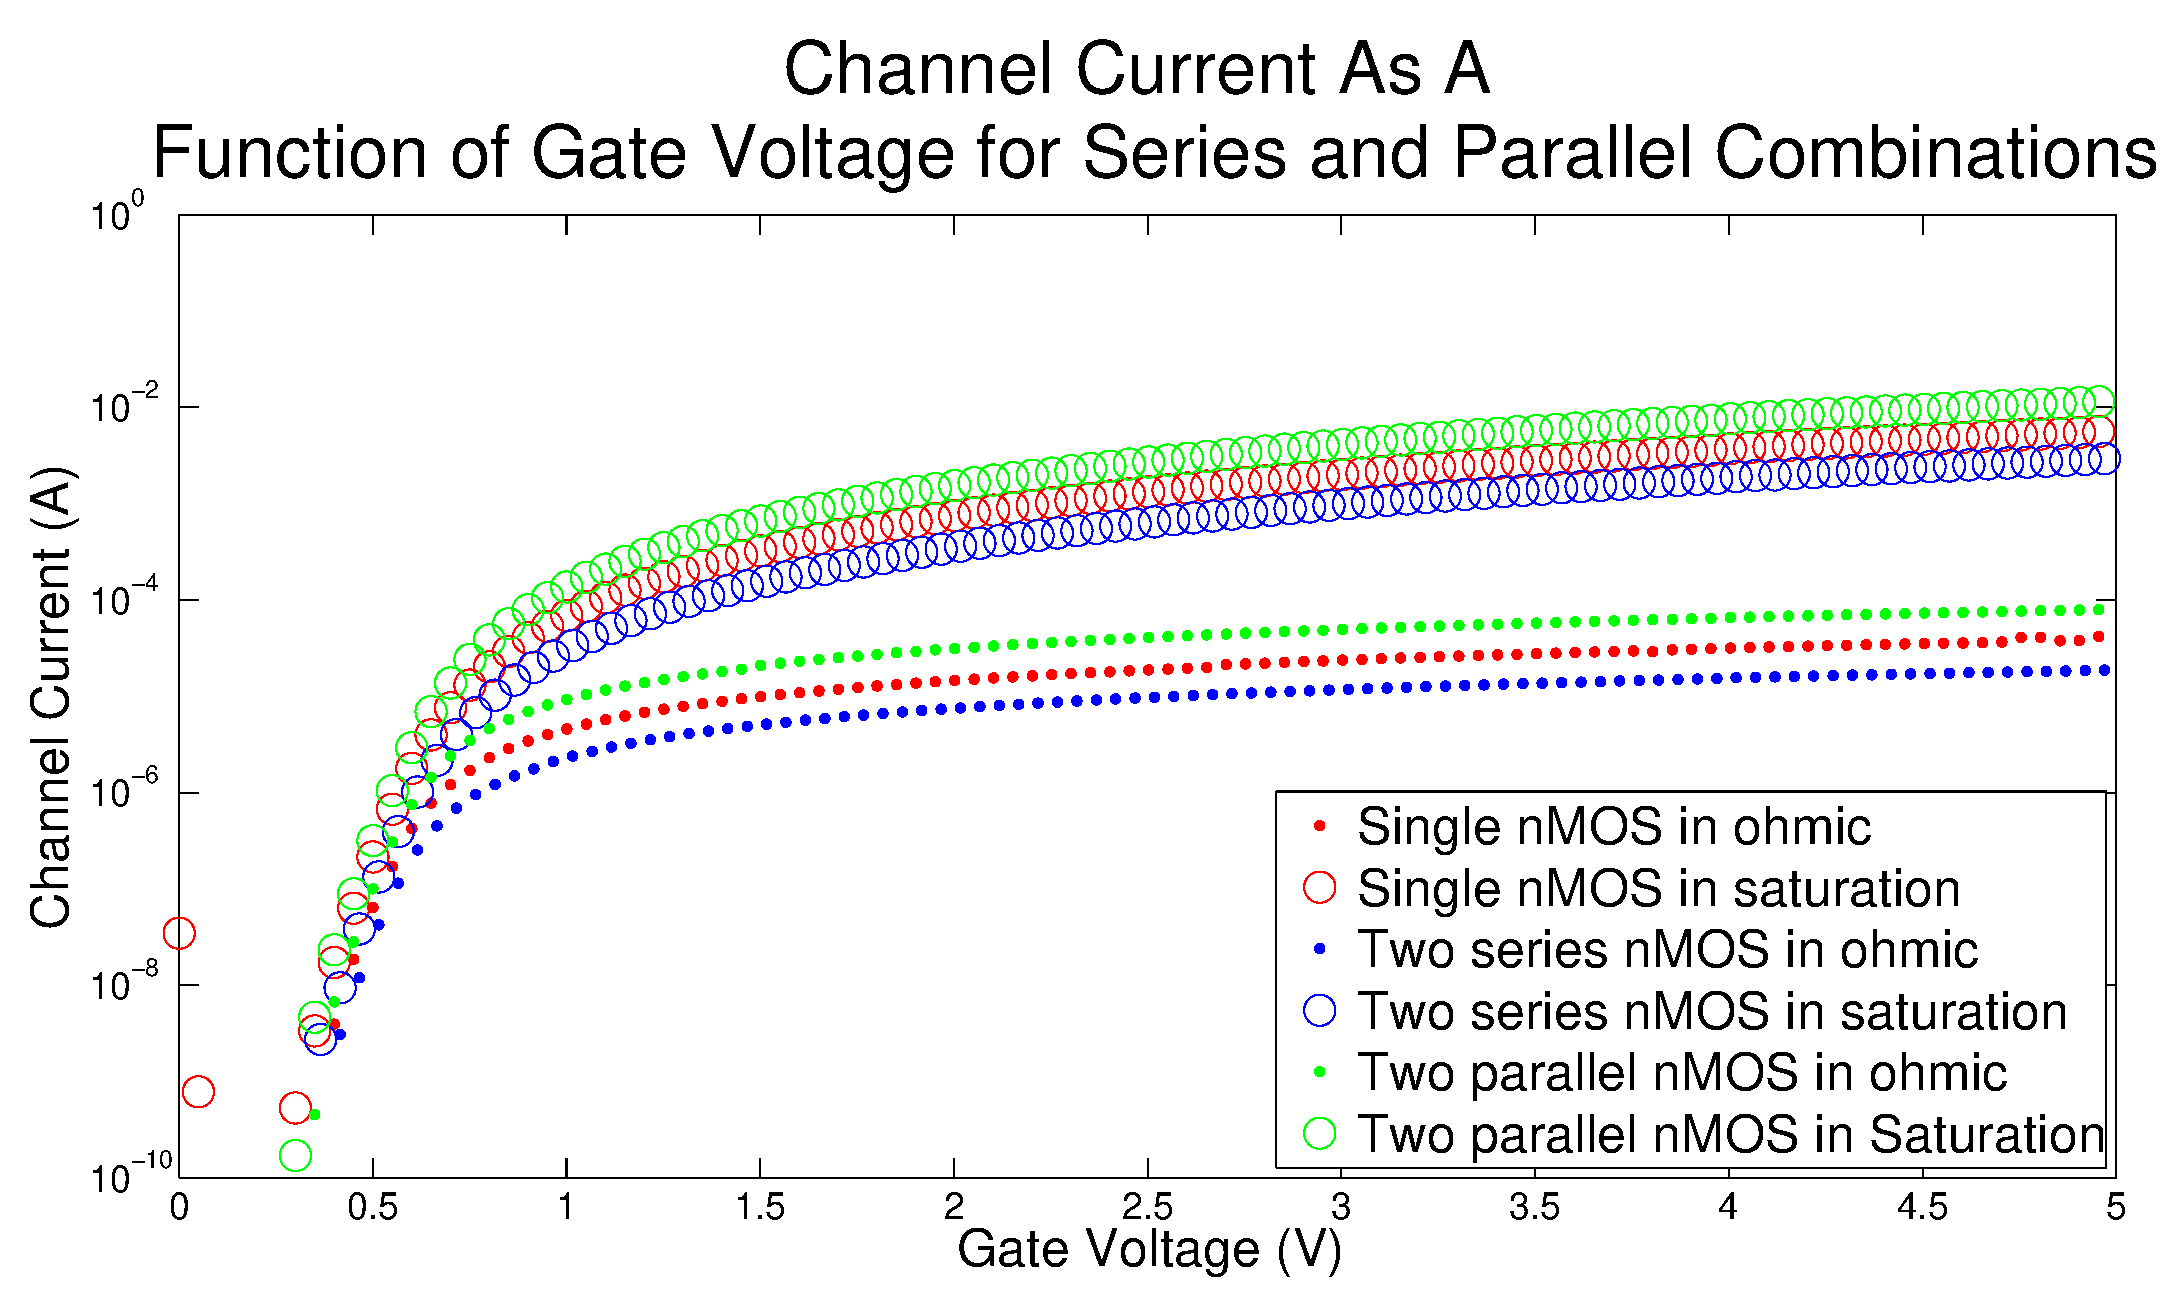
\includegraphics[width=\linewidth]{../Figures/Experiment2Currents.eps}
\caption{Note that after SMU is able to accurately measure current, after the channel current increases past roughly $10^{-8}$, the three different arrangements are separated by a constant distance in logspace, and thus appear to differ by a constant factor.}
\label{fig:exp2currents}
\end{figure}

By analyzing Figure \ref{fig:exp2currents}, we can see that the series, parallel and single curves appear to be offset by a linear distance in logspace, thus indicating that there is a linear factor between the relationships. 

In order to find the true relationship, we explored the ratio of both the series and parallel combination of \nMOS transistors with the same \Vg, \Vd, \Vs and \Vb, plotting these ratios as a function of the gate voltage, \Vg, below in Figure \ref{fig:exp2ratios}. 
In the strong inversion region, the ratio between both the series and parallel combinations to that of a single transistor is consistently, $0.5$ and $2$, respectively. That is to say, from our experimental data, a pair of series transistors sinks half the current as a single transistor, and a pair of transistors in parallel sinks twice the current of a single transistor, when matched.

\begin{figure}[H]
\centering
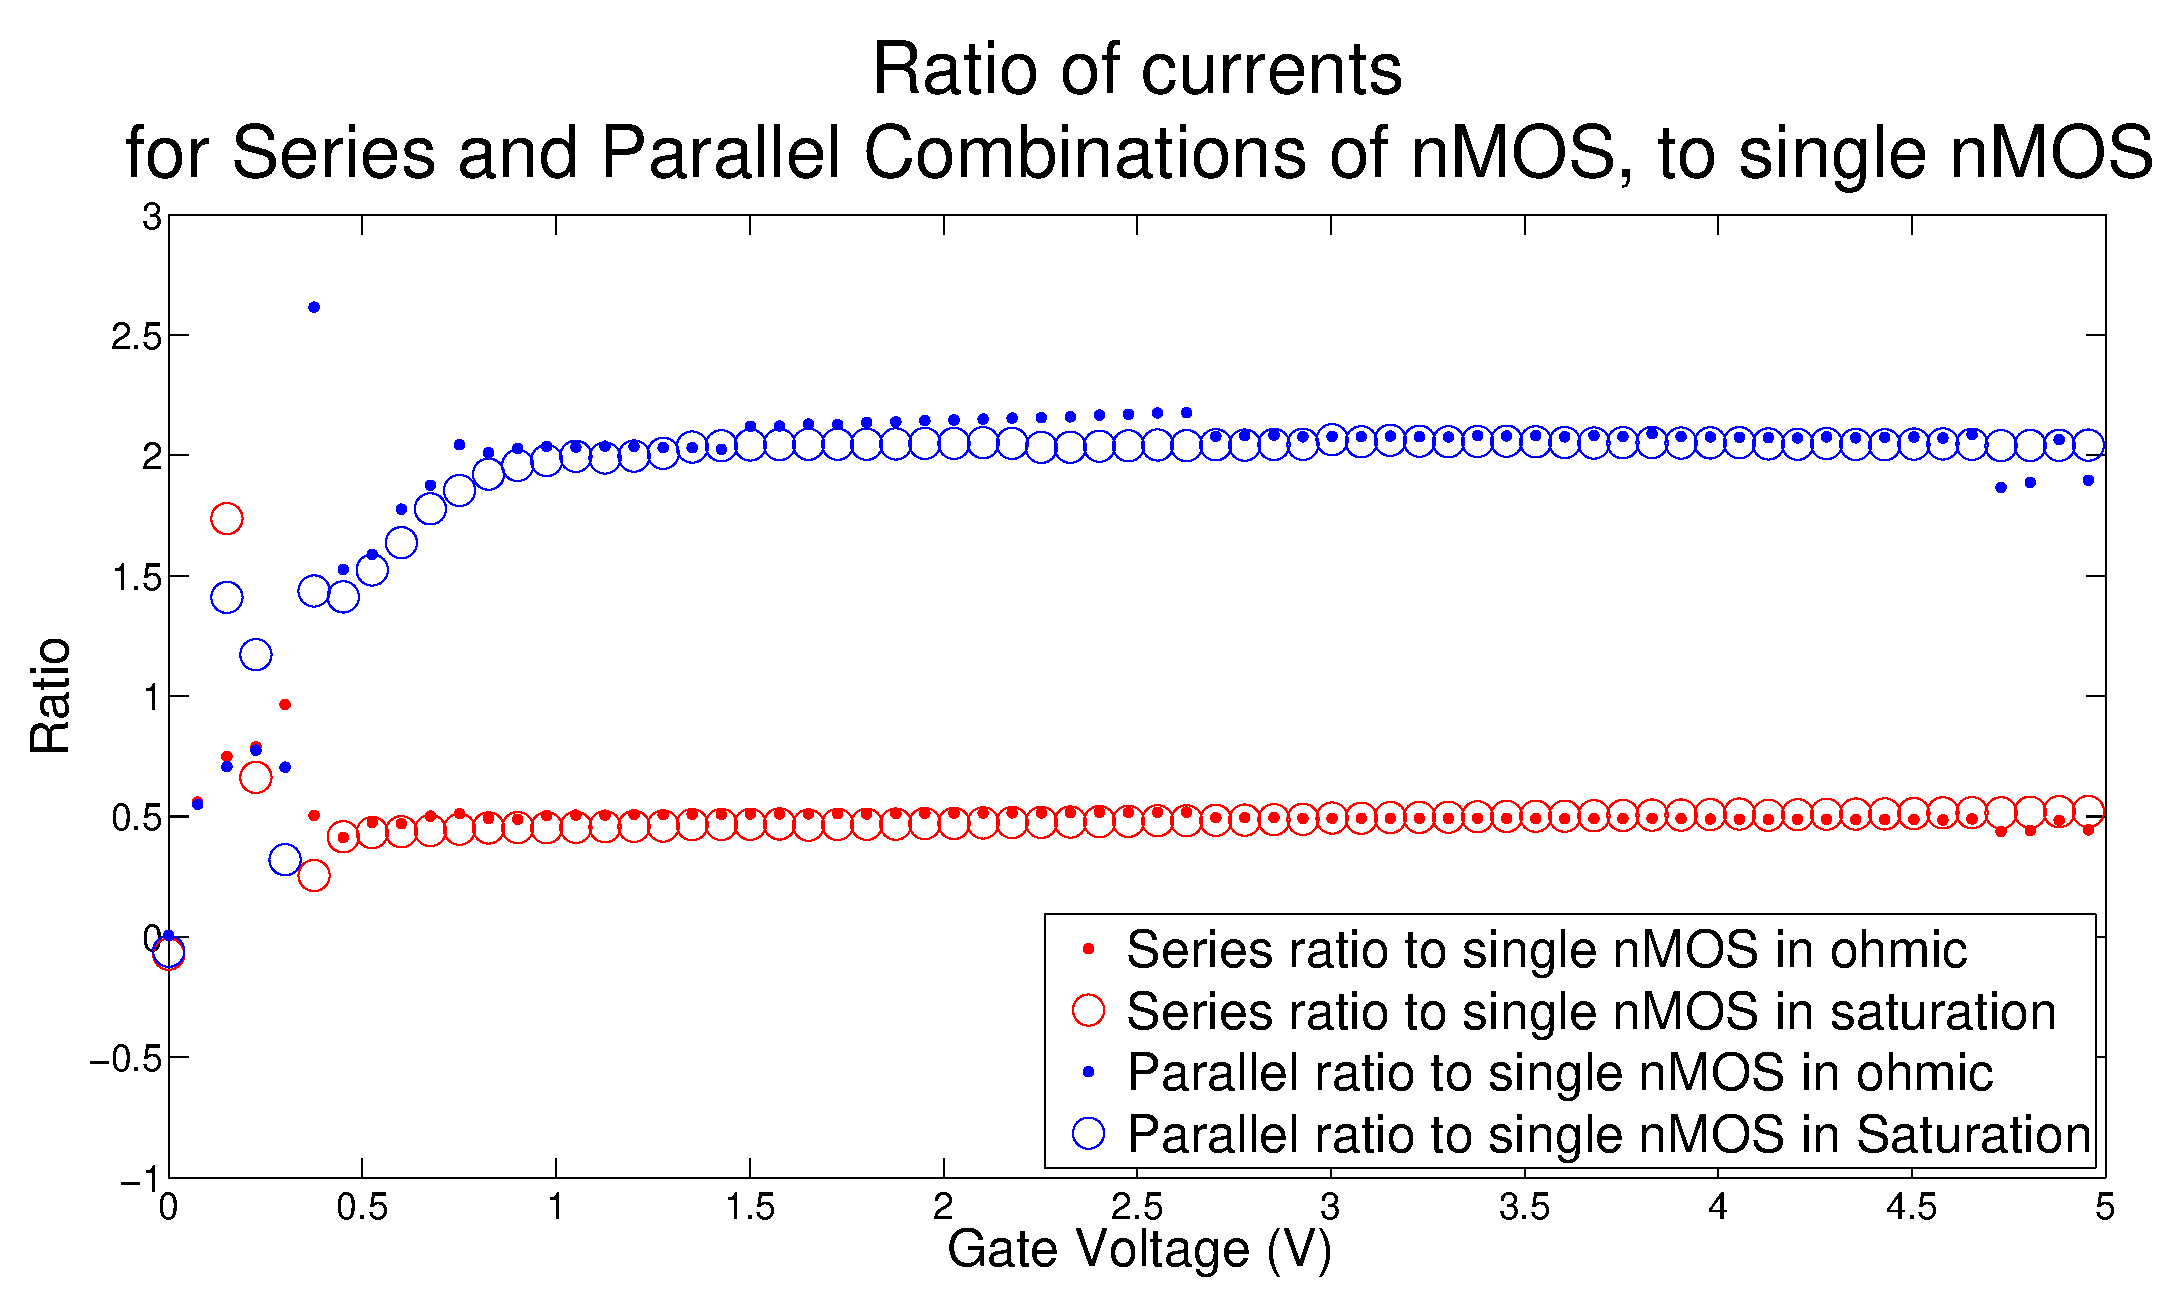
\includegraphics[width=\linewidth]{../Figures/Experiment2Ratios.eps}
\caption{After the two curves stabilize, past roughly $0.75V$, the ratio between both series and parallel combinations to a single \nMOS is consistent, and produces the expected value; a pair of \nMOS transistors in series has half the current of one, and a pair of \nMOS transistors in parallel has twice the current as a single transistors.}
\label{fig:exp2ratios}
\end{figure}

Meanwhile, in the weak inversion region of operation, the series combination of transistors much better maintains a consistent ratio, quickly approaching a 1:2 ratio as the SMU is able to accurately measure current. Before this value, we believe a combination of SMU error at low current and measurement of leakage current cause the deviation. 


On the other hand, the parallel combination does not approach the ratio of 2:1 until $1V$. We believe it takes this parallel combination much longer because the leakage current measured is effectively double. Further, since different individual transistors were used in this test, it may be due to the relatively large deviation of Transistor 2, shown in Figure \ref{fig:exp1fig2}. We used Transistor 2 in the parallel combination, and since it had a higher strength factor than the other three resistors, more current would flow through it, thus making the parallel pair have a ratio closer to 1:1, rather than the 2:1 it eventually achieves, as the voltage increases.



